\begin{figure}
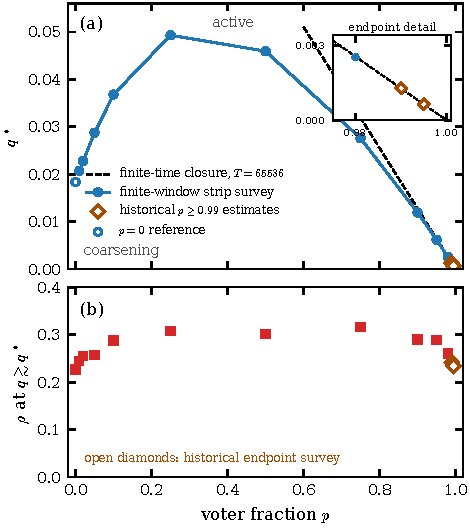
\includegraphics[width=\columnwidth]{figs/fig_phase}
\caption{(a) Finite-window invasion survey at $\alpha=1/2$ from strip
fronts (Table~\ref{S-tab:line}), with the refined $p=1/2$ operational
reference. The open blue circle denotes the $p=0$ reference with
additional frozen states. Open orange diamonds identify the historical
$p=0.99$ and 0.995 estimates; the inset enlarges the endpoint region.
The dashed line is the finite-time closure
$q_f(T)=c_f(T)\alpha(1-p)$ at $T=65536$, where $c_f=0.2553$.
(b) Time-weighted density at the actual nearby probabilities $q_\rho$
in Table~\ref{S-tab:line}, with equal run weights and one standard error.
Open orange diamonds again mark the historical endpoint survey.
The $p\ge0.99$ summaries combine nearby probabilities and observation
horizons. Longer trajectories at $p=0.995$, $q=0.000640$ show substantial
late decay in Fig.~\ref{fig:gpu_near20m}; the historical endpoint markers
do not locate a limiting transition or its density jump.}
\label{fig:phase}
\end{figure}
